\documentclass[11pt,a4paper,notitlepage]{report} % notitlepage doesnt reset pagenumber on abstract
\usepackage[portuguese]{babel}
\usepackage[latin1,utf8]{inputenc} %utf8 for linux
\usepackage[T1]{fontenc}
\usepackage{hyperref}
%\usepackage[a4paper, pdftex, bookmarks, colorlinks, linkcolor=black, urlcolor=blue]{hyperref} %por linkcolor=cor para ter os links com cor.
\usepackage[a4paper,left=3cm,right=2.5cm,top=3cm,bottom=2.5cm]{geometry}
%\usepackage[margin=10pt,font=small,labelfont=bf]{caption}
%\usepackage{graphicx}
\usepackage{float} % for floating objects
%\usepackage{multirow}
\usepackage{array}
\usepackage{amsfonts}
\usepackage{amsmath}
\usepackage{mathtools}
%\usepackage[table]{xcolor}
\usepackage[section]{placeins} % para os floats nao ultraparassem a section em que sao criados
%\usepackage[portuguese]{nomencl} % para a lista de nomenclaturas
%\makenomenclature
%\usepackage[toc,page]{appendix}
\usepackage{algpseudocode} % for algorithms
\usepackage{algorithm} % for algorithms
\usepackage[titletoc]{appendix} % as seen here: http://stackoverflow.com/questions/5690679/add-appendix-before-a-in-thesis-toc
%\usepackage[nottoc]{tocbibind} % para meter a bibliografia no toc
\usepackage{enumerate} % para o enumerate a), b)
\usepackage{listings}
\usepackage[margin=10pt,font=small,labelfont=bf]{caption}
\usepackage{color}
\usepackage{todonotes} % Mark­ing things to do in a LATEX doc­u­ment
%
\newenvironment{definition}[1][Definição]{\begin{trivlist}
\item[\hskip \labelsep {\bfseries #1}]}{\end{trivlist}}
\newenvironment{example}[1][Exemplo]{\begin{trivlist}
\item[\hskip \labelsep {\bfseries #1}]}{\end{trivlist}}
%
%%%%%%%%%%%%%%%%%%%%%%%%%%%%%
% new commands
%%%%%%%%%%%%%%%%%%%%%%%%%%%%%
\newcommand{\HRule}{\rule{\linewidth}{0.5mm}} % para a capa
\newcommand{\sage}{\texttt{Sage}}
\newcommand{\RingLPN}{\textsf{Ring-LPN}}
\newcommand{\RingLPNR}{\textsf{Ring-LPN}$\mathsf{^R}$}
\newcommand{\RingLPNRtau}{\textsf{Ring-LPN}$\mathsf{^R_\tau}$}
%
%
% mudar algorithm para algoritmo
\floatname{algorithm}{Algoritmo}
\renewcommand{\algorithmicrequire}{\textbf{Input:}}
\renewcommand{\algorithmicensure}{\textbf{Output:}}
% mudar appendices para anexos
\renewcommand{\appendixtocname}{Apêndices}
\renewcommand{\appendixpagename}{Apêndices}
% floating algorithms
\newfloat{algorithm}{t}{lop}
% mudar list of nomenclatures para palavras chave
%\renewcommand{\nomname}{Palavras Chave}
%
% listings
\definecolor{dkgreen}{rgb}{0,0.6,0}
\definecolor{gray}{rgb}{0.5,0.5,0.5}
\definecolor{mauve}{rgb}{0.58,0,0.82}
\renewcommand{\lstlistingname}{Código}
\lstdefinestyle{sage}{
  frame=tb,
  language=Python,
  tabsize=2,
  breaklines=true,
  breakatwhitespace=true,
  basicstyle={\footnotesize\ttfamily},
  aboveskip=3mm,
  belowskip=3mm,
  numberstyle=\tiny\color{gray},
  keywordstyle=\color{blue},
  commentstyle=\color{dkgreen},
  stringstyle=\color{mauve},
  showstringspaces=false,
  captionpos=t,
  %morecomment=[is]{\#}{ } % could be used to hide comments
}
% \include includes the file in a new page
% \input include the file in the current page
% \chapter[short description]{long description}
% use \and when using more than one author
% to use bibtex: \cite{citation_name}
%
%
\begin{document}
\pagenumbering{roman}
\begin{titlepage}

\begin{center}

% Upper part of the page

\includegraphics[width=0.25\textwidth]{img/um-eng}\\[1cm]

\textsc{\LARGE Universidade do Minho\\Departamento de Informática}\\[1cm]

\textsc{\Large Criptografia e Segurança dos Sistemas de Informação}\\[0.5cm]
\textsc{\Large Projecto Integrador II\\2012/2013}\\[0.25cm]
\textsc{\textit{Milestone} 1}\\[0.5cm]


% Title
\HRule \\[0.4cm]
{ \huge \bfseries Post quantum authentication}
\HRule \\[1.5cm]
%
% Author and supervisor
\begin{minipage}[t]{0.4\textwidth}
\begin{flushleft} \large
pg22797 Milton \textsc{Nunes}\\
%[1.5cm]
pg22815 Nuno \textsc{Carvalho}\\
%[1.5cm]
\end{flushleft}
\end{minipage}
\begin{minipage}[t]{0.4\textwidth}
\begin{flushright} \large
\textbf{Supervisor:}\\
Prof. Manuel Bernardo \textsc{Barbosa}
\end{flushright}
\end{minipage}

\vfill

% Bottom of the page

{\large Abril de \the\year}

\end{center}
\newpage
\thispagestyle{empty} % no pagenumber on this page
\begin{center}
  \vspace*{\fill}
  \begin{tabular}{m{3cm} m{0.5cm}}
%  %\begin{tabular}{c}
%    % demasiado escaxe LOL
%    %\includegraphics[width=0.55\textwidth]{../img/grupo/escaxe}\\
%    %(esq para dir) Milton Nunes, Nuno Carvalho, Rafael Remondes\\
    Milton Nunes & 
\includegraphics[width=0.15\textwidth]{img/grupo/milton}\\ \\
    Nuno Carvalho & 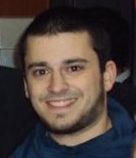
\includegraphics[width=0.15\textwidth]{img/grupo/teddy}\\ \\
  \end{tabular}
  \vspace*{\fill}
\end{center}
\end{titlepage}

%
%\maketitle
\newpage
%
% the abstract
\begin{abstract}
\thispagestyle{plain} % pagenumber on abstract page
Com o eventual aparecimento dos computadores quânticos, os esquemas de assinaturas baseados no problema da factorização ou do logaritmo discreto tornar-se-ão inúteis. Posto isto, tornou-se imperativo procurar esquemas de assinaturas digitais que se apresentassem como alternativas viáveis. Esta procura levou a que se chegassem a esquemas baseados em reticulados, que se revelaram uma alternativa válida ao problema que se pretendia resolver e que proporcionaram avanços significativos em várias áreas da criptografia. \\
Este Projecto Integrador pretende abordar e explorar a aplicabilidade de esquemas criptográficos de autenticação de mensagens baseados em reticulados. Neste relatório será apresentado todo o trabalho de análise e estudo efectuado sobre as duas publicações sugeridas \cite{lapin,lattice_sig}.\\
Do estudo efectuado para esta primeira \textit{milestone}, resultou um pequeno protótipo em \sage\ do protocolo Lapin descrito em \cite{lapin}. Além disso, são também apresentados os objectivos que se esperam alcançar no desenvolvimento deste projecto.

\end{abstract}
\newpage
%\input{nomenclature}
%\printnomenclature
%\newpage
%table of contents
\tableofcontents
\newpage
%
\pagenumbering{arabic}
\chapter{Introdução}
\section{Objectivos}
Nesta primeira fase pretende-se estudar o protocolo de autenticação Lapin. Para isso, vamos implementar um pequeno protótipo em \sage, visto que já utilizámos \sage\ para o primeiro Projecto Integrador. Depois de implementado o protótipo, é necessário escolher uma linguagem para a implementação do protocolo.\\
As opções consideradas para a implementação do protocolo eram \textsf{C}, \textsf{C++} e \textsf{Java}. Estamos mais confortáveis em \textsf{Java}, mas visto que o Lapin é especialmente orientado para dispositivos \textsf{low-cost}, decidimos usar \textsf{C}.\\
Para esta primeira fase também efectuámos um estudo das operações aritmétricas mais eficientes, usando apenas operações binárias. Estas operações até poderão ser inicialmente criadas em \sage, com o objectivo de conhecer e perceber melhor os algoritmos das mesmas.\\
No resto do presente documento, apresenta-se todo o estudo e trabalho desenvolvido para esta primeira fase. 
\chapter{Lapin -- Estudo}
\section{Descrição}
O protocolo Lapin apresentado em \cite{lapin} consiste num protocolo de autenticação baseado no problema \RingLPN\ (\textit{Ring variant of the Learning Parity with Noise}). Este protocolo, constituído por apenas dois \textit{rounds} e seguro contra ataques activos, tem uma complexidade de comunicação bastante pequena, pelo que é indicado para dispositivos \textit{low-cost} ou em cenários onde os recursos são limitados.\\
Em comparação com outros protocolos, que fazem uso de cifras por blocos como por exemplo o AES, o Lapin mostra-se como uma boa alternativa. Em casos onde se possuam algumas centenas de bytes de memória não-volátil, onde se poderão guardar alguns resultados pré-computados, o protocolo apenas é apenas duas vezes mais lento que o AES, mas em compensação, tem cerca de dez vezes menos código do que o AES.\\
%%%%%%%%%%%%%%
% Conceitos
%%%%%%%%%%%%%%
\section{Conceitos}
%%%%%%%%%%%%%%%
% Polinomios
%%%%%%%%%%%%%%%
\subsection{Polinómios}
O protocolo baseia-se essencialmente em operações sobre polinómios binários, ou seja, polinómios em $\mathbb{F}_2[x]$. Todos os polinómios do protocolo pertencem ao anel $\mathbb{F}_2[x]/f(x)$, sendo que um elemento deste anel tem grau máximo $deg(f)-1$. No âmbito deste projecto, serão considerados dois anéis $\mathsf{R} = \mathbb{F}_2[x]/f(x)$: um anel em que $f(x)$ é irredutível e outro em que $f(x)$ é factorizável em $m$ polinómios distintos. Denota-se por $\widehat{a}$ a representação CRT (Teorema Chinês dos Restos) do polinómio $a$ em relação aos $m$ factores do $f(x)$ factorizável, ou seja, $\widehat{a} = (a \bmod{f_1}, \dotsc, a \bmod{f_m})$\\
%%%%%%%%%%%%%%%%%%%%%%%%
% Distributions
%%%%%%%%%%%%%%%%%%%%%%%%
\subsection{Distribuições}
Uma distribuição \textsf{D} sobre determinado domínio representa-se sob a forma de $r \longleftarrow_{\$} \mathsf{D}$, sendo $r$ o valor gerado de acordo com a distribuição \textsf{D}. Denomina-se uma distribuição uniforme sobre o domínio \textsf{Y} como \textsf{U(Y)}. Seja a distribuição de \textsf{Bernoulli},  $\textsf{Ber}_{\tau}$ sobre $\mathbb{F}_2$ com o parâmetro $\tau \in\ ]0,1/2[$. Para um anel polinómio $\mathsf{R} = \mathbb{F}_2[x]/f(x)$, a distribuição $\textsf{Ber}_{\tau}^\mathsf{R}$ denota a distribuição sobre polinómios de $\mathsf{R}$, para os quais os coeficientes são determinados independentemente de $\textsf{Ber}_{\tau}$. Para um anel $\mathsf{R}$ e um polinómio $s \in \mathsf{R}$, representa-se $\Lambda_{\tau}^{\mathsf{R},s}$ como uma distribuição sobre $\mathsf{R} \times \mathsf{R}$ sendo as amostragens obtidas através dos polinómios $r \longleftarrow_{\$} \mathsf{U(R)}$ e $e \longleftarrow_{\$} \mathsf{Ber}_{\tau}^\mathsf{R}$, cujo resultado é o seguinte \textit{output}: $(r, rs+e)$.
%%%%%%%%%%%%%%%%
% RingLPN e LPN
%%%%%%%%%%%%%%%%
\subsection{Ring Learning Parity with Noise (\RingLPN) e Learning Parity with Noise (\textsf{LPN})}
A segurança do protocolo depende problema do \textsf{Ring-LPN} que se trata de uma expansão do problema \textsf{LPN} para anéis. Este problema pode também ser visto como uma instanciação particular de um outro problema com grande ligação aos reticulados, o \textsf{Ring-LWE} (\textit{Learning with Errors over Rings}).\\
A diferença entre os dois problemas reside na diferença entre dois possíveis oráculos. O primeiro oráculo gera aleatoriamente um vector secreto $s \in \mathbb{F}_2^n$ que é usado produzir a resposta. No problema \textsf{LPN}, cada chamada do oráculo produz, de forma uniforme, uma matriz aleatória $A \in \mathbb{F}_2^{n \times n}$ e um vector $As + e = t \in \mathbb{F}_2^n$, onde $e$ é um vector de $\mathbb{F}_2^n$ em que cada entrada é um valor aleatório gerado independentemente pela distribuição de \textit{Bernoulli} com a probabilidade de 1 usando o parâmetro público $\tau$ entre $0$ e $1 \setminus 2$. O segundo oráculo gera uma matriz $A \in \mathbb{F}_2^{n \times n}$ aleatória de forma uniforme e um vector aleatório $t \in \mathbb{F}_2^n$ de forma igualmente uniforme.\\
A diferença entre o \textsf{LPN} e o \textsf{Ring-LPN} está na geração da matriz $A$, em ambos os oráculos. Enquanto no problema \textsf{LPN} todas as entradas são geradas de forma uniforme e independente, no problema \textsf{Ring-LPN} apenas a primeira coluna é gerada dessa forma em $\mathbb{F}_2^n$, sendo que as restantes colunas dependem da primeira e do anel subjacente $\mathsf{R} = \mathbb{F}_2[x]/f(x)$. De assinalar ainda que a suposição $\textsf{Ring-LPN}^\mathsf{R}$ indica que é difícil distinguir entre os \textit{outputs} dos dois oráculos.\\
O problema \textsf{LPN} é bastante usado em criptografia como uma suposição difícil, ao contrário do \textsf{Ring-LPN}. Contudo, uma publicação recente demonstra que o problema \textsf{Ring-LWE} é tão difícil quanto resolver quanticamente o pior caso de um pequeno vector de reticulados. Por sua vez, o 
\textsf{Ring-LPN} é bastante semelhante ao problema \textsf{Ring-LWE}.
%%%%%%%%%%%%%%%%%%%
% Funcionamento
%%%%%%%%%%%%%%%%%%%
\section{Funcionamento}\label{lapin:protocol}
O protocolo é definido sobre o anel $\mathsf{R} = \mathbb{F}_2[x]/f(x)$ e envolve um \textit{mapping} adequado $\pi : \{0,1\}^{\lambda} \rightarrow \mathsf{R}$. Este \textit{mapping} deve ser definido de tal forma que $\forall \, c, c' \in \{0,1\}^\lambda$ tem-se que $\pi(c) - \pi(c') \in \mathsf{R} \setminus \mathsf{R}^\star$ sse $c = c'$.\\
Descreve-se de seguida o funcionamento do protocolo: 
\begin{center}
  \begin{tabular}{| l  c  r |}
    \hline
     \multicolumn{3}{| l |}{Parâmetros Públicos: $\mathsf{R}, \pi : \{0,1\}^\lambda$ $\rightarrow \mathsf{R}, \tau, \tau'$} \\
     \multicolumn{1}{| l }{Chave Privada: $s, s' \in \mathsf{R}$}  &  & \\
    &  & \\
    &  &  \\
     \multicolumn{1}{| c }{\textsf{Tag}  $\mathcal{T}$} &  & \multicolumn{1}{ c |}{\textsf{Leitor}  $\mathcal{R}$} \\
     &  & \\
     & $\xleftarrow{c}$ & \multicolumn{1}{l |}{$c \leftarrow_{\$} \{0,1\}^\lambda$} \\ 
    $r \leftarrow_{\$} \mathsf{R}^*$;  $e \longleftarrow_{\$} \mathsf{Ber}_{\tau}^R \in \mathsf{R}$ &  &  \\ 
    $z := r \cdot (s \cdot \pi(c) + s') + e$ & $\xrightarrow{(r,z)}$ &  \\
     &  & \multicolumn{1}{ l |}{se $r \notin \mathsf{R}^\star$ retorna \textsf{reject}} \\
     &  & \multicolumn{1}{ l |}{$e' := z - r \cdot (s \cdot \pi(c) + s')$} \\
     &  & \multicolumn{1}{ l |}{se $\mathsf{wt}(e') > n \cdot \tau'$ retorna \textsf{reject}} \\
     &  & \multicolumn{1}{ l |}{retorna \textsf{accept}}\\
    \hline
  \end{tabular}
\end{center}
%
\begin{description}
  \item[Parâmetros públicos] $\tau, \tau'$ representam constantes (definidas mais adiante), $n$ depende do parâmetro de segurança $\lambda$:
    \begin{itemize}
      \item Anel $\mathsf{R} = \mathbb{F}_2[x]/f(x)$ com $deg(f) = n$
      \item \textit{Mapping} $\pi : \{0,1\}^\lambda \rightarrow \mathsf{R}$
      \item Parâmetro da distribuição de Bernoulli $\tau \in \mathbb{R}$ e \textit{threshold} aceitação $\tau' \in \mathbb{R}$ tal que $0 < \tau < \tau' < 1/2$
      %\item Parâmetro da distribuição de Bernoulli $0 < \tau < 1/2$, $\tau \in \mathbb{R}$
      %\item \textit{Threshold} de aceitação $\tau < \tau' < 1/2$, $\tau' \in \mathbb{R}$
    \end{itemize}
  \item[Geração de chaves] Algoritmo $\mathsf{KeyGen}(1^\lambda)$ amostra $s, s' \longleftarrow_{\$} \mathsf{R}$ e retorna $s, s'$ como a chave privada
  \item[Protocolo de autenticação] O Leitor $\mathcal{R}$ e a \textit{Tag} $\mathcal{T}$ partilham a chave secreta $s, s' \in \mathsf{R}$. Para que $\mathcal{T}$ seja autenticada por $\mathcal{R}$, ambos executam os seguintes passos:
    \begin{enumerate}
      \item $\mathcal{R}$ gera um \textit{challenge} $c \longleftarrow_{\$} \{0,1\}^\lambda$. \textbf{$\mathbf{\mathcal{R}}$ envia $\mathbf{c}$ para $\mathbf{\mathcal{T}}$}
      \item $\mathcal{R}$ gera $r \longleftarrow_{\$} \mathsf{R}$, $e \longleftarrow_{\$} \mathsf{Ber^{R}_\tau}$ e calcula $z = r \cdot (s \cdot \pi(c) + s') + e$. \textbf{$\mathbf{\mathcal{T}}$ envia o par $\mathbf{(r,z)}$ para $\mathbf{\mathcal{R}}$}
      \item $\mathcal{T}$ recebe o par $(r,z)$ e:
        \begin{itemize}
          \item se $r \notin \mathsf{R}^\star$, retorna \textsf{reject} e protocolo termina;
          \item calcula $e' = z - r \cdot (s \cdot \pi(c) + s')$;
          \item se $\mathsf{wt}(e') > n \cdot \tau'$, retorna \textsf{reject} e protocolo termina\footnote{$\mathsf{wt}(e)$ representa o \textit{hamming weight} de uma \textit{string} binária $e$, ou seja, o número de bits 1 em $e$};
          \item retorna \textsf{accept}
        \end{itemize}
    \end{enumerate}
\end{description}
%%%%%%%%%%%
% Redutivel
%%%%%%%%%%%
\subsection{Polinómio redutível}
Por questões de eficiência, por vezes é melhor utilizar um polinómio $f(x)$ que seja redutível sobre $\mathbb{F}_2$. Isto permite-nos utilizar a representação CRT dos elementos de $\mathbb{F}_2[x]/f(x)$ para efectuar multiplicações que se tornam muitos mais eficientes quando em CRT.\\
Se o polinómio é factorizável em $\prod_{i=1}^{m} f_i$, então é possível tentar resolver o problema do \RingLPN\ módulo um qualquer $f_i$, em vez de $f$. Sendo que o $deg(f_i) < deg(f)$, resolver o \RingLPN\ torna-se mais fácil.\\
A implementação do protocolo através da utilização de um polinómio redutível permite-nos tirar vantagens da aritmética baseada no Teorema Chinês dos Restos.\\
Na implementação é definido o anel $\mathsf{R} = \mathbb{F}_2[x]/f(x)$, e escolhido o polinómio redutível $f$ como o produto de $m = 5$ polinómios irredutíveis:
$$
\begin{array}{c c c c c c c c c c c}
  f_1 &=& x^{127} &+& x^{8} &+& x^{7} &+& x^{3} &+& 1 \\
  f_2 &=& x^{126} &+& x^{9} &+& x^{6} &+& x^{5} &+& 1 \\
  f_3 &=& x^{125} &+& x^{9} &+& x^{7} &+& x^{4} &+& 1 \\
  f_4 &=& x^{122} &+& x^{7} &+& x^{4} &+& x^{3} &+& 1 \\
  f_5 &=& x^{121} &+& x^{8} &+& x^{6} &+& x     &+& 1 \\
\end{array}
$$
Por isso, $deg(f) = n = 621$. É definido $\tau = 1/6$ e $\tau' = 0.29$ de forma a obter um erro de solidez mínimo $\varepsilon_{ms} \approx c(\tau', 1/2)^{-n} \le 2^{-82}$ e um erro de integridade $\varepsilon_{c} \le 2^{-42}$. O melhor ataque conhecido sobre \RingLPNRtau\ tem como parâmetro a complexidade $>2^{80}$.\\
O \textit{mapping} $\pi : \{0,1\}^{80} \rightarrow \mathsf{R}$ é definido no Algoritmo~\ref{alg:pi_irreduc}. Cada $v_i$ pode ser visto como a representação dos coeficientes de um polinómio em $\mathbb{F}_2[x]/f_i(x)$. O \textit{mapping} $\pi$ está representado na forma CRT. De referir ainda que, para $c, c^\star \in \{0,1\}^{80}$, temos que $\pi(c) - \pi(c^\star) \in \mathsf{R} \setminus \mathsf{R}^\star$ sse $c = c^\star$ e por isso $\pi$ é adequado para \textsf{R}.\\
\begin{algorithm}
  \caption{\textit{Mapping} $\pi$ para o anel $\mathsf{R} = \mathbb{F}_2[x]/f(x)$, no caso em que $f(x)$ é irredutível}\label{alg:pi_irreduc}

  \begin{algorithmic}
    \Require $c \in \{0, 1\}^{80}$
    \Ensure $\pi = (v_1, \dotsc, v_5)$
    \For {$i = 1$ to $5$}
    \State    $toPad = deg(f_i) - 80$
    \State    $v_i = padding(c, toPad)$
    \EndFor 
    \State \Return $v$
  \end{algorithmic}
\end{algorithm}
%%%%%%%%%%%
% Irredutivel
%%%%%%%%%%%
\subsection{Polinómio irredutível}
Quando $f(x)$ é irredutível em $\mathbb{F}_2$, o anel $\mathbb{F}_2[x]/f(x)$ é um corpo. Para estes anéis, não são conhecidos algoritmos capazes de tirar partido da estrutura algébrica adicionada a esta instância particular do \RingLPN. Desta forma, o algoritmo conhecido mais eficiente para resolver este problema é usado para resolver o \textsf{LPN}.\\
A complexidade computacional do problema \textsf{LPN} baseia-se no tamanho de \textit{n} e na distribuição de ruído $\mathsf{Ber_\tau}$. Intuitivamente, quanto maior for \textit{n} e $\tau$ mais próximo de $1/2$, mais difícil se torna o problema.\\
Habitualmente, são considerados como valores de $\tau$ valores constantes entre $0.05$ e $0.25$. Para tais valores de $\tau$, o algoritmo assimptótico mais rápido para a resolução do problema \textsf{LPN} demora $2^{\Omega(n/log\ n)}$ e requer aproxidamente $2^{\Omega(n/log\ n)}$ amostragens do oráculo \textsf{LPN}. No caso do número de amostragens ser menor, o algoritmo, naturalmente, tem uma performance inferior. No protocolo o número de amostragens disponíveis para o adversário é limitado a $n$ vezes o número de execuções. Então, assumindo que o adversário tem acesso a um número limitado de amostragens, é mais difícil quebrar o protocolo de autenticação do que resolver o problema \RingLPN.\\
Para definir o corpo $\mathsf{F} = \mathbb{F}_2[x]/f(x)$ foi escolhido o polinómio irredutível:
$$
  f(x)  =  x^{532} + x + 1 \\
$$
Por isso com grau $n = 532$, e definidos $\tau = 1/8$ e $\tau' = 0.27$ que permite obter um erro de solidez mínimo $\varepsilon_{ms} \approx c(\tau', 1/2)^{-n} \le 2^{-80}$ e um erro de integridade $\varepsilon_{c} \le 2^{-55}$.\\
De acordo com análises citadas na publicação, o algoritmo mais rápido na resolução do problema \textsf{LPN} de dimensão $532$ com $\tau = 1/8$ requer $2^{77}$ de memória para o resolver quando é dado aproxidamente o mesmo número de amostras. Dado que a dimensão é pouco maior e o número de amostras limitado, é razoável assumir que esta instância tem segurança de $80$ bits.\\
O \textit{mapping} $\pi : \{0,1\}^{80} \rightarrow \mathsf{F}$ é definido no Algoritmo~\ref{alg:pi_irreduc}. Dado que $\pi$ descrito é injectivo e \textsf{F} é um corpo, o \textit{mapping} $\pi$ é adequado para \textsf{F}.
\begin{algorithm}
  \caption{\textit{Mapping} $\pi$ para o corpo $\mathsf{F} = \mathbb{F}_2[x]/f(x)$, no caso em que $f(x)$ é redutível}\label{alg:pi_reduc}

  \begin{algorithmic}
    \Require $c \in \{0, 1\}^{80} = (c_1, \dotsc, c_16)$, com cada $c_j$ um número de 5 bits entre 1 e 31
    \Ensure $(v_1, \dotsc, v_{16})$ os 16 coeficientes não nulos.
    \For {$j = 1$ to $16$}
    \State    $v_i = 16 \cdot (j - 1) + c_j$
    \EndFor
    \State \Return $v$
  \end{algorithmic}
\end{algorithm}

\chapter{Lapin -- Implementação}
\section{Representações e operações em \sage}
Antes de partir para a implementação do protocolo em \textsf{C}, decidimos criar um pequeno protótipo em \sage. A grande vantagem é o facto de o \sage\ ter diversas classes definidas para a representação de polinómios, sendo que as operações usuais de soma, multiplicação ou módulo estão já implementadas, poupando-nos algum tempo que pode ser utilizado para melhor perceber o funcionamento do protocolo. \\
Apresentamos neste secção algumas das classes usadas, e como implementar algumas das operações do protocolo.\\
Para se representar $\mathbb{F}_2[x]$ usa-se:
\begin{lstlisting}[style=sage]
F = PolynomialRing(GF(2), 'x')
\end{lstlisting}
Para declarar um polinómio não basta declará-lo com, por exemplo, \verb|x^2 + x|, pois o tipo da variável \verb|x| é uma \verb|Expression| do \sage. Posto isto, é preciso declarar a variável \verb|x| para que o \sage\ saiba que está a lidar com polinómios e não com simples \verb|Expressions| \sage. Sendo assim, para declarar $f(x) = x^7 + x + 1$ faz-se:
\begin{lstlisting}[style=sage]
sage: x = F.gen()
sage: f = x**7 + x + 1
\end{lstlisting}
É desta forma que vamos definir todos os polinómios em \sage. Agora é possível efectuar operações sobre polinómios. Seguem alguns exemplos, em que todas as operações são efectuadas em $\mathbb{F}_2[x]$:
\begin{lstlisting}[style=sage]
sage: g = x**5 + x**2 + x + 1
sage: f+g
x^7 + x^5 + x^2
sage: f*g
x^12 + x^9 + x^8 + x^7 + x^6 + x^5 + x^3 + 1
sage: f.mod(g)
x^4 + x^3 + x^2 + x + 1
sage: 
\end{lstlisting}
Tendo bem definido como se tratariam dos polinómios, é necessário representar o anel \textsf{R}. Usando como exemplo o anel $\mathbb{R}_2[x]/f(x)$ tem-se:
\begin{lstlisting}[style=sage]
sage: R = R.quotient_ring(f, 'x')
sage: R.random_element()
x^6 + x^5 + x^4 + x
# CAREFUL: type of this R.random_element() doesn't support mod operations, so we have to convert it to type Polynomial_GF2X
sage: type(R.random_element())
sage.rings.polynomial.polynomial_quotient_ring_element.Polynomial
QuotientRing_generic_with_category.element_class
sage: type(binToPoly(polyToBin(R.random_element(), x), x)
sage.rings.polynomial.polynomial_gf2x.Polynomial_GF2X
\end{lstlisting}
Note-se que as funções \verb|binToPoly| e \verb|polyToBin| estão definias no Anexo~\ref{}
Como também vamos ter de trabalhar com polinómios em CRT, vamos criar um exemplo de um anel \textsf{R} com um $f(x) = x^8 + x^6 + x^4 + x^3 + x$ factorizável em três polinómios $x$, $x^3 + x + 1$ e $x^4 + x + 1$ e com algumas operações em CRT:
% aquele f = reduce() e o mesmo que o foldl do haskell
\begin{lstlisting}[style=sage]
sage: fi = [x, x**3 + x + 1, x**4 + x + 1]; f = reduce(operator.mul, fi, 1)
sage: R = F.quotient_ring(f, 'x')
sage: z = R.random_element();
# convert z to Polynomial_GF2X
...
sage: zCRT = map(lambda m : z.mod(m), fi) ; zCRT
[1, x^2, x^2 + 1]
sage: CRT_list(zCRT, fi) == z
True
sage: w = R.random_element()
# convert w to Polynomial_GF2X
...
sage: wCRT = map(lambda m : w.mod(m), fi) ; wCRT
[1, x + 1, x^3 + x + 1]
# perform w*z (mod f)
sage: tmp1 = zip(wCRT, fi); tmp2 = zip(zCRT, fi)
sage: wzCRT=map(lambda ((x1, y1), (x2, y2)) : (x1*x2).mod(y1), zip(tmp1,tmp2))
sage: CRT_list(wzCRT, fi) == (w*z).mod(f)
True
\end{lstlisting}
Como também vamos precisar de trabalhar com a string de bits $c \in \{0, 1\}^\lambda$, seguem-se os comandos para a criar, converter para representação inteira e para fazer \textit{padding}:
\begin{lstlisting}[style=sage]
sage: c = bin(getrandbits(80))[2:].zfill(80) ; Integer(c,2)
64597992717886966981887
# type of c is str and len(c) = 80
sage: ''.join(['0' * 5], c) # pad c with 5 bits
\end{lstlisting}
%%%%%%%%%%%%%%%%%%%%%%%%%%%%%%%%%%%%%%%
% Protocolo em Sage
%%%%%%%%%%%%%%%%%%%%%%%%%%%%%%%%%%%%%%%
\section{Algumas operações em \sage}
Tendo já conhecimento dos métodos apresentados anteriormente, é relativamente fácil concluir a implementação do Lapin no \sage. Apresentámos agora alguns dos métodos e funções com maior relevância. Todo o código pode ser consultado no Anexo~\ref{appendix:lapin}.\\
Decidimos dividir a implementação do Lapin em três classes:
\begin{description}
  \item[Lapin] contém a definição dos parâmetros do protocolo, conforme os recomendados em \cite{lapin}. Contém todas as operações do protocolo apresentadas em \ref{lapin:protocol}, à excepção do \textit{mapping} $\pi$;
  \item[Reducible] contém todas as operações comuns ao protocolo no caso em que $f$ é redutível. É aqui definido o \textit{mapping} $\pi$ e o anel \textsf{R}
  \item[Irreducible] contém todas as operações comuns ao protocolo no caso em que $f$ é irredutível. É aqui definido o \textit{mapping} $\pi$ e o corpo \textsf{F}
\end{description}
As operações auxiliares comuns não estão em nenhuma classe de forma a possibilitar a sua utilização por todas as classes/funções do protocolo. Exemplo de tais funções são as que implementam somas e multiplicações em CRT ou operações binárias.\\
De seguida apresenta-se o passo 2 do protocolo no caso em que $f$ é redutível:
\begin{lstlisting}[style=sage]
# method of Reducible class
def tag_step2(self, c):
  # ....
  
  # list of factors of f
  fi = self.protocol.fi

  r = reduceToCRT(self.protocol.genR(), fi)
  e = reduceToCRT(self.protocol.genE(self.tau), fi)
  # keys in crt form
  (s1, s2) = (reduceToCRT(self.key1, fi), reduceToCRT(self.key2, fi))
  pi = self.protocol.pimapping(c)

  z = addCRT(multCRT(r, addCRT(multCRT(s1, pi, fi), s2, fi), fi), e, fi)
  return (r, z)
  
# ...
# function, not a method of any class
def reduceToCRT(a, fi):
  return map(lambda f : a.mod(f), fi)
\end{lstlisting}
O método \verb|pimapping| é a implementação do Algoritmo~\ref{alg:pi_irreduc}.\\
O passo 3 consiste na verificação. Eis a sua implementação para o caso em que $f$ é irredutível:
\begin{lstlisting}[style=sage]
# method of Irreducible class
def reader_step3(self, c, r, z):
  # ....
  
  # list of factors of f
  fi = self.protocol.fi

  (r1, z1) = (CRT_list(r, fi), CRT_list(z, fi))
  if r1.gcd(self.protocol.f) != 1:
    print "reject R*"
    return False
  pi = CRT_list(self.protocol.pimapping(c), fi)

  e2 = (z1 - r1 * (self.key1 * pi + self.key2)).mod(self.protocol.f)

  if e2.hamming_weight() > (self.n * self.tau2):
    print "reject wt"
  return False

  print "accept"
  return True
\end{lstlisting}
\section{Polinómios binários}
Como pretendermos implementar de raíz o protocolo em \textsf{C}, é necessário perceber como funcionam as operações sobre polinómios ao mais baixo nível, ou seja, apenas com a utilização de operações sobre bits.\\
Neste capítulo pretende-se explicar como implementar as operações aritmétricas mais comuns sobre polinómios de forma eficiente. Até ao momento, só efectuámos a análise de duas operações: soma e multiplicação. A soma é de relativamente fácil percepção e implementação, mas na multiplicação demorámos mais tempo a perceber como realmente funciona. Devido a este facto, não nos é possível apresentar ainda a implementação das outras operações aritmétricas necessárias, tais como o módulo e máximo divisor comum (\textsf{gcd}).\\
\subsection{Representação binária}
De forma a que as operações com polinómios sejam o mais eficiente possível, é necessário trabalhar sobre a sua representação binária, em vez de os representar com simples inteiros. Neste capítulo descreve-se a representação usada na implementação do Lapin.\\
Uma forma bastante simples de representar polinómios é colocar o bit menos significativo do lado direito, sendo a tradução de um polinómio para binário a seguinte:
$$
x^7 + x^4 + x^2 + x + 1 \Leftrightarrow 1 0 0 1 0 1 1 1
$$
O bit mais significativo representa o monómio $x^7$, enquanto que o menos significativo representa o $1$.\\
Mas esta forma, por si só, não é a mais apropriada para implementar as operações aritmétricas em \textit{software}. Em \cite{lapin}, o autor refere-se a um método de multiplicação de polinómios mais eficiente, descrito em \cite{Hankerson:2003:GEC:940321}. Antes de descrever esses métodos, é necessário introduzir uma nova forma de representar polinómios binários.\\
Nesta nova forma, assume-se que a máquina tem um arquitectura de $W$-bits, em que $W$ é um múltiplo de 8. Um polinómio passa a ser visto como um conjunto de palavras de $W$ bits, em que o bit menos significativo continua a estar do lado direito.\\
Assume-se que existe o polinómio irredutível $f(x)$ com $deg(f) = m$. Todos os elementos $a(x)$ de $\mathbb{F}_2[x]/f(x)$ tem grau menor ou igual a $m-1$. Cada elemento $a(x)$ tem associada a representação descrita anteriormente, ou seja, é o vector binário $a = (a_{m-1}, a_m, \dotsc, a_1, a_0)$ de tamanho $m$. Considere-se $t = \lceil m/W \rceil$ e $s = Wt - m$. O vector binário $a$ pode ser guardado num \textit{array} de $t$ palavras de $W$ bits: $A = A[t-1], A[t], \dotsc, A[1], A[0]$. Os $s$ bits mais à direita de $A[t-1]$ nunca são usados (estão sempre a 0).\\
A partir de agora vamos usar sempre esta última representação para tratar de polinómios.\\
%%%%%%%%%%%%%%
% soma
%%%%%%%%%%%%%%
\subsection{Soma}
A soma de dois polinómios pode ser vista como um simples XOR entre as palavras dos dois polinómios, sendo efectuado o XOR palavra a palavra, bit a bit. No Algoritmo~\ref{alg:bin_add} descreve-se este processo.
\begin{algorithm}
  \caption{Soma de palavras binárias de $W$ bits}\label{alg:bin_add}

  \begin{algorithmic}
    \Require Polinómios $a(x)$ e $b(x)$ de grau menor ou igual a $m-1$
    \Ensure Polinómio $c(x) = a(x) + b(x)$
    \For {$i = 0$ to $t - 1$}
    \State    $C[i] = A[i] \oplus B[i]$
    \EndFor
    \State \Return c
  \end{algorithmic}
\end{algorithm}
%%%%%%%%%%%%%%%%%%%
% multplicacao
%%%%%%%%%%%%%%%%%%%
\subsection{Multiplicação de dois polinómios binários}
Ao contrário da soma descrita no Algoritmo~\ref{alg:bin_add}, a multiplicação de polinómios já não é tão simples. Em \cite{lapin}, sugere-se a utilização do o método \textit{right-to-left comb} descrito em \cite{Hankerson:2003:GEC:940321} por ser o mais eficiente.\\
Tal como para a soma, um polinómio é visto como $t$ palavras de $W$ bits. Em cada iteração conhece-se o resultado de $b(x) \cdot x^k$ para $k \in [0, W-1]$, logo, $b(x) \cdot x^{Wj+k}$ pode facilmente ser obtido adicionando $j$ palavras nulas (a zero) à direita do vector que representa $b(x) \cdot x^k$. Tal como o próprio nome indica, as palavras de $A$ são percorridas da direita para a esquerda. Quando se tem um array $C = C[n],\dotsc,C[1],C[0]$, denota-se por $C\{j\} = C[n],\dotsc,C[j+1],C[j]$ como o array truncado.
\begin{algorithm}
  \caption{Método \textit{Right-to-left comb} para a multiplicação de dois polinómios}\label{alg:right_to_left}
  \begin{algorithmic}
    \Require Polinómios $a(x)$ e $b(x)$ de grau menos ou igual a $m-1$
    \Ensure Polinómio $c(x) = a(x) \cdot b(x)$
    \State $C = 0$
    \For {$k = 0$ to $W - 1$}
      \For{$j = 0$ to $t - 1$}
        \If{$k$-ésimo bit de $A[j]$ é $1$}
        %%%%%%%%%%%%%%%%%%%%%%%%%%%%%%%%%%%%%%%%%%
        %% fodasse, isto ta mal. corrigir isto
        %%%%%%%%%%%%%%%%%%%%%%%%%%%%%%%%%%%%%%%%%%
        \State Adicionar $B$ a $C\{j\}$
        \State $c(x) = c(x) + b(x) \cdot x^{Wj + k}$ % Wj + k ou Wj??
        \State $C = C\{j\} + B$
        \EndIf
      \EndFor
      \If{$k \neq (W - 1)$}
      \State $b(x) = b(x) \cdot x$
      \State $B = B \cdot x$
      \EndIf
    \EndFor
    \State \Return C
  \end{algorithmic}
\end{algorithm}

%\chapter{\textit{Lattice Signatures Without Trapdoors}}
%Infelizmente, não foi feito um estudo muito rigoroso deste protocolo. 
\chapter{Conclusão}
%%%%%%%%%%%
% Conclusao
%%%%%%%%%%%
Baseado no estudo efectuado sobre o protocolo de autenticação Lapin, pode-se afirmar que o mesmo é uma opção viável e segura para implementar em sistemas \textit{low-cost} e com recursos limitados, em que se pretenda um protocolo com pequena complexidade comunicacional. A análise de \cite{lapin} permitiu também verificar a utilidade de algumas operações realizadas sobre polinómios que permitem alcançar resultados muito mais eficientes comparativamente às operações realizadas da forma habitual. De assinalar ainda que a utilização da suposição \textsf{Ring-LPN}, apesar de ainda não ser um problema muito utilizado em criptografia, vem demonstrar que a sua utilização pode vir a aumentar, especialmente no âmbito das construções de esquemas \textit{low-cost}.\\
Relativamente ao esquema de assinaturas baseadas em \textit{Lattices} foi possível concluir que este é solução bastante interessante e com bastante potencial, contudo as limitações para os casos que conseguimos de facto testar apresentaram resultados que não são ainda aceitáveis para uma utilização prática consistente e eficiente. De ressalvar também que a nossa análise não é extensível a todos os casos referidos na publicação, sendo que os restantes são baseados em problemas diferentes dos testados, e por isso os resultados poderão ser diferentes. Claramente esta é uma área de investigação em evolução e com grande potencial.
%%%%%%%%%%%%%%%%%%%%
% Implementação
%%%%%%%%%%%%%%%%%%%%
\section{Resultados de implementação e trabalho futuro}
A implementação do Lapin acabou por não se tornar muito complexa, sendo bastante simples perceber o funcionamento do protocolo olhando apenas para o código. No entanto as operações aritmétricas sobre polinómios acabaram por ser a parte mais complicada de implementar, sendo que a função de redução modular \verb|poly_mod| pode ser melhorada. Outra opção que com certeza irá aumentar a eficiência do protocolo será a utilização dos algoritmos de redução modular mais rápidos (\textit{fast modulo reduction} \cite{Hankerson:2003:GEC:940321}). Resta-nos terminar a implementação do algoritmo de Euclides estendido, do CRT e a utilização do gerador \textit{urandom} para geração aleatória de polinómios. Além disso, há operações que podem sofrer pequenas optimizações. Entendemos ainda que seria relevante modificar a nossa implementação de forma a que se tornasse em algo menos académico e mais direccionado à utilização prática no dia-a-dia em dispositivos mais restringidos.\\
Em relação às assinaturas digitais baseadas em reticulados seria extremamente interessante aprofundar o estudo relativamente às distribuições, o que influenciaria directamente a geração do vector \textbf{y} e também a \textit{rejection sampling}. Mais precisamente, seria interessante implementar o algoritmo de amostragem gaussiana apresentado em \cite{galbraith2012efficient}. Esta questão das distribuições revelou-se algo complexa e não foi possível abordá-las mais profundamente, mas acreditamos que o protocolo se revelaria mais eficiente com essas modificações.\\ 
Gostaríamos também de conseguir aprofundar o nosso conhecimento sobre a teoria dos reticulados, dado que à partida para este projecto o nosso conhecimento sobre a matéria era praticamente zero. De qualquer forma, achamos que os resultados obtidos foram bastante mais do que satisfatórios.
%
%
% bibtex
\bibliographystyle{plain}
\nocite{*} % Show all Bib-entries
% Note the lack of whitespace between the commas and the next bib file.
\bibliography{bib/articles,bib/books,bib/www}
%
\appendix
\appendixpage
\addappheadtotoc
\chapter{Lapin em \sage}\label{appendix:lapin}
\section{Protocolo Lapin, classe principal}
\lstinputlisting[style=sage,caption={Implementação do protocolo Lapin em \sage}]{appendix/lapin.sage}

\section{Operações do Lapin, com o polinómio redutível}
\lstinputlisting[style=sage,caption={Operações do protocolo, com o polinómio redutível, em \sage}]{appendix/lapin-reducible.sage}
\
\section{Operações do Lapin, com o polinómio irredutível}
\lstinputlisting[style=sage,caption={Operações do protocolo, com o polinómio redutível, em \sage}]{appendix/lapin-irreducible.sage}

\section{Funções comuns usadas pelo Lapin}
\lstinputlisting[style=sage,caption={Funções usadas pelo protocolo Lapin em \sage}]{appendix/lapin-functions.sage}
\chapter{Operações binárias em \sage}\label{appendix:bin-ops}
\section{Operações com polinómios binários}
De seguida apresenta-se a soma de polinómios binários. Infelizemente, não conseguimos terminar a tempo a implementação da multiplicação de polinómios, mas neste apêndice encontram-se a maior parte das funções necessárias à sua implementação.
\lstinputlisting[style=sage,caption={Implementação da soma de polinómios binários. Contém também algumas funções auxiliares para conversão de polinómios para binário e vice-versa.}]{appendix/bin-operations.sage}
%\chapter{Outro anexo}
\end{document}
